\subsection{Protein solubility}
% The Gibb's phase rule describes the state of a system at equilibrium and is given by 

% \begin{equation}
%     f + p = c + 2
% \end{equation}

% where $c$ is the number of components, $p$ is the number of phases and $f$ is the degree of freedom. For a two phase system (solid and liquid) at constant pressure and temperature, with two components (solute and solvent for example, protein and water), $f = 0$. This means the amount of protein in solution phase no longer depends upon the total amount of protein in the system and remains constant \cite{arakawa19853}. Thermodynamically, the chemical potential of protein in solid phase and liquid phase are now equal. The physical solubility, thus, can be defined as the concentration of protein in a saturated solution which is in equilibrium with the solid phase. Solubility has units of moles per liter ($m/L$) and often, for convenience, written in grams per liter ($g/L$). 


% This physical solubility of a protein depends on the experimental conditions such as temperature, pH, ionic concentration \cite{Kramer2012-wk}. This might lead to the variability of results across various experimental conditions. Hence, 
Solubility is defined as the proportion of the supernatant fraction, obtained after the centrifuging the the translation mixture, to the uncentrifuged total protein \cite{Niwa2009-ye}. It ranges from $0\%$ to $130\%$ with solubility less than $30\%$ categorised as aggregation-prone and greater than $70\%$ are highly soluble. Several \textit{intrinsic} features of the protein itself such as molecular weight, flexibility, hydrophobicity, isoelectric point and structural propensities are also known to influence solubility \cite{Wilkinson1991-zp, Chiti2003-zk, Tartaglia2004-wm, Diaz2010-md}. Sometimes these intrinsic features are modified by doing either mutagenesis or truncation, which might assist in improving solubility. Several solubility enhancing tags are also available for example, thioredoxin (TRX), maltose binding protein (MBP), small ubiquitin-related modifier (SUMO) and glutathione S-transferase (GST). Although, the exact mechanisms of how these tags work is still unclear, it is proposed that they might act like a chaperone and assist in correct folding of the target protein or add charges which decreases the overall aggregation propensity \cite{Costa2014-oe}.

\subsubsection{Intrinsic properties of a protein}
Intrinsic properties are derived from different properties of the residues inside the poly-peptide chain. The commonly used intrinsic properties of proteins are described below.

\paragraph{Hydrophobicity}
Water soluble proteins fold such that the hydrophilic parts are exposed and can form hydrogen bonds with the water molecules whereas the hydrophobic parts are buried in the core. This hydrophobic effect is thought to be responsible for protein solubility \cite{tanford1978hydrophobic}. Several scales have been proposed to measure the hydrophobicity of residues \cite{Kyte1982-qn, abraham1987extension, janin1979surface, rose1985hydrophobicity}. However, none of these scales can fully model the full range of behaviour of residues \cite{charton1982structural}. 


We will use Kyte-Doolittle's scale \cite{Kyte1982-qn} for representative purposes. In this scale, residues are given a hydropathy score such that positive scores represent hydrophobicity and negative score represent hydrophilicity. The magnitude of score represents the strength. For example: isoleucine (I) is given 4.5 and is the most hydrophobic residue, where as  arginine (R) is given -4.5 and is the most hydrophilic residue. Using these scores, a hydropathy plot for a given polypeptide can be drawn (Fig. \ref{fig:hydrophobicity_flexibility_plot}). Hydropathy plot can be used to examine the hydrophobicity of protein region of interest. Using hydrophobic effect, we can then infer whether the residue is buried or located on the surface. Furthermore, the overall hydrophobicity of the protein can be determined by averaging the hydropathy scores across the polypeptide chain to obtain the GRand AVerages of hydropathY (GRAVY) score.


\begin{figure}[htbp!]
\center
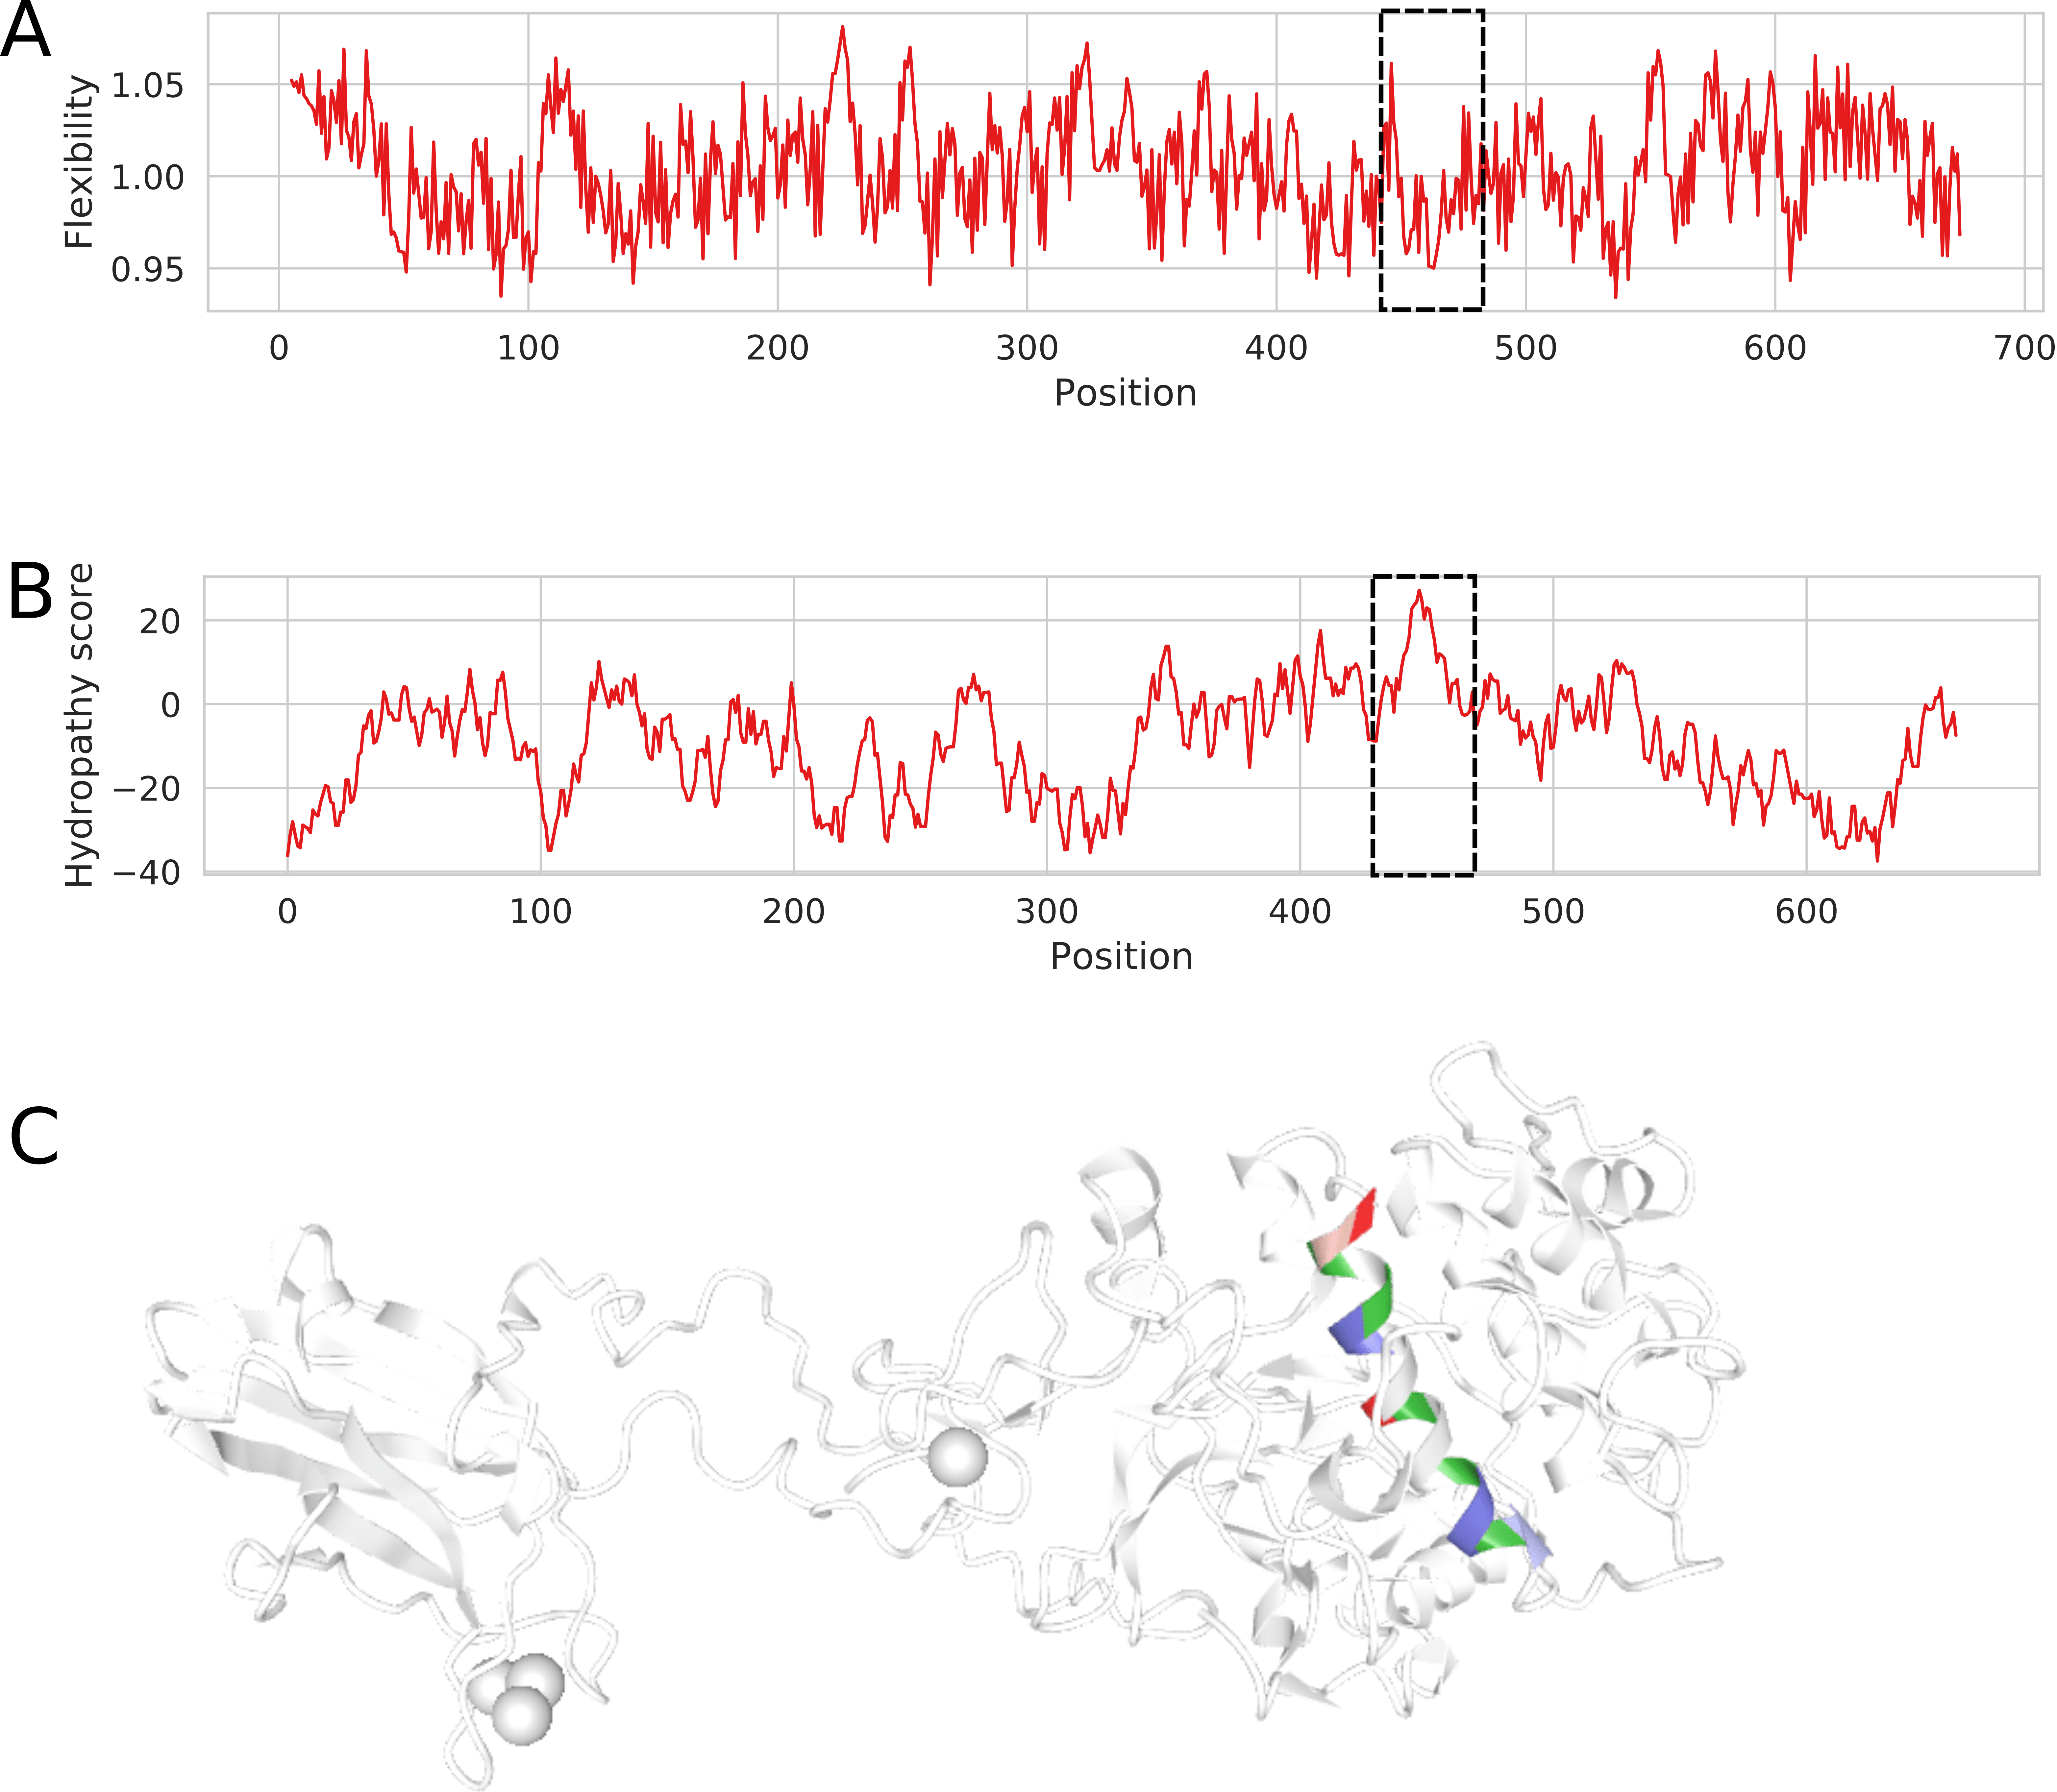
\includegraphics[width=1\textwidth]{chapters/Introduction/Figures/flex_and_hydrop.png}
\caption[Profiles of KPC1\_DROME (UniProtKB P05130).]{\textbf{Profiles of KPC1\_DROME (UniProtKB P05130)}. 
\textbf{(A)} Flexibility plot generated using normalised B-factors from Vihinen et al. (1994), with a sliding window of 9 residues. For these normalised B-factors, values greater than one are regarded to be flexible and values less than one are rigid. \textbf{(B)} Hydropathy plot generated using Kyte-Doolittle's hydrophobicity scale, with a sliding window of 19 residues. For illustration, the hydropathy and flexibility of residues at around position $440$ to $470$ (shown by dotted box) are positive and rigid. This indicates the presence of an alpha helix which is supported by the actual 3D structure \textbf{(C)}. The coloured helix is the region $440$ to $470$.  }%the List of Figures because of the *}
\label{fig:hydrophobicity_flexibility_plot}
\end{figure}


% \begin{figure}[htbp!]
% \center
% 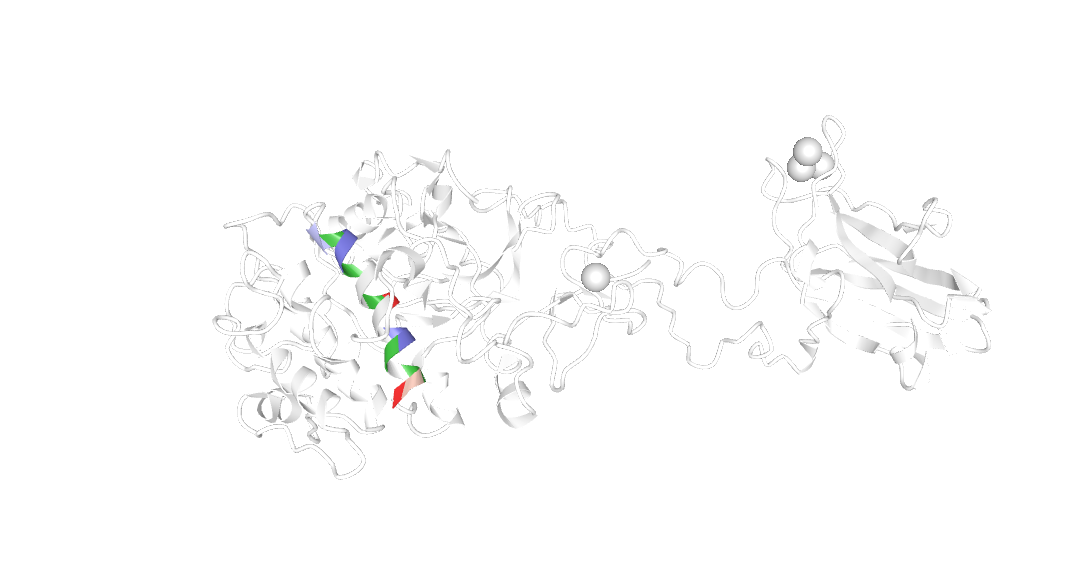
\includegraphics[width=1\textwidth]{chapters/Introduction/Figures/kpc1_drome.png}
% \caption{\textbf{3D structure of KPC1\_DROME (UniProtKB P05130)}. The highlighted helix runs from position $448$ to $467$. The presence of this helix can be inferred by the hydropathy plot (Fig \ref{fig:hydrophobicity_plot}) and the flexibility profile plot (Fig. \ref{fig:flexibility_plot}). }%the List of Figures because of the *}
% \label{fig:3dplot_kpc1_drome}
% \end{figure}


\paragraph{Isoelectric point}
The net charge of a protein at a given pH depends on acid dissociative constant (pKa) of ionisable groups such as amine and carboxyl group. At a certain pH, the amount of negative and positive charge are equal, resulting a zero net charge. This pH is called the isoelectric point (pI). The net charge is positive at pH below pI and negative at pH above pI \cite{shaw2001effect}. Since there are no net charges, the solubility of a protein is minimum at the isoelectric point.

\paragraph{Instability index}
Guruprasad et. al \cite{guruprasad1990correlation} found that the distribution of certain dipeptides on stable and unstable protein is different. Based on 12 unstable and 32 stable proteins, they assigned a weight called dipeptide instability weight value (DIWV) for all dipeptides. The instability index (II) is then given by equation \ref{eqn:instability_index}.

\begin{equation}
    II = \frac{10}{L}\sum_{i=1}^{L-1}DIWV(x_i y_{i+1})
    \label{eqn:instability_index}
\end{equation}

where $L$ is the length of the sequence and $x_i y_{i+1}$ is a dipeptide.

%%%http://pd.chem.ucl.ac.uk/pdnn/refine3/adps.htm
%%Biomolecular Crystallography: Principles, Practice, and Application : page 641

\paragraph{Flexibility}
Protein molecules are dynamic and are inherently flexible due to the motion of the constituent atoms \cite{vihinen1994accuracy, alvarez2014relationship, teilum2009functional}. The structural flexibility of a protein can be inferred by using B-factors \cite{vihinen1994accuracy, Karplus1985-ea, Smith2003-gb}.


The B-factor (Equation \ref{eqn:bfactor}) or temperature factor of the atoms in a crystalline structure is the measure of mean squared displacement vibration around their mean position $(u = \langle (x-x_0)^2 \rangle)$, where $x$ is the displacement of the atom from its mean position $x_0$. B-factor thus reflects the \textit{orderedness} of the crystal lattice and subsequent uncertainty in X-ray scattering structure determination \cite{Schlessinger2005-ps, Carugo2018-ka, Bramer2018-dh}. It has unit of $\r{A}^2$.


\begin{equation}
    B = 8\pi^2 u
    \label{eqn:bfactor}
\end{equation}

To understand the effect of the B-factor, we define a quantity $f$ called the atomic scattering factor as:

\begin{equation}
    f = \frac{amplitude\ of\ wave\ scattered\ by\ an\ atom}{amplitude\ of\ wave\ scattered\ by\ one\ electron}
\end{equation}

Atomic scattering factor after taking into account of the motion of atom becomes:

\begin{equation}
    f_B = f\cdot e^{-B(sin\ \theta /\lambda)^2}
\end{equation}

where $\theta$ is the Bragg angle and $\lambda$ is the wavelength of the wave. Thus, we see that B-factor attenuates the amplitude of wave scattered by an atom (Figure \ref{fig:bfactors} ).

% \begin{figure}[htbp!]
% \center
% 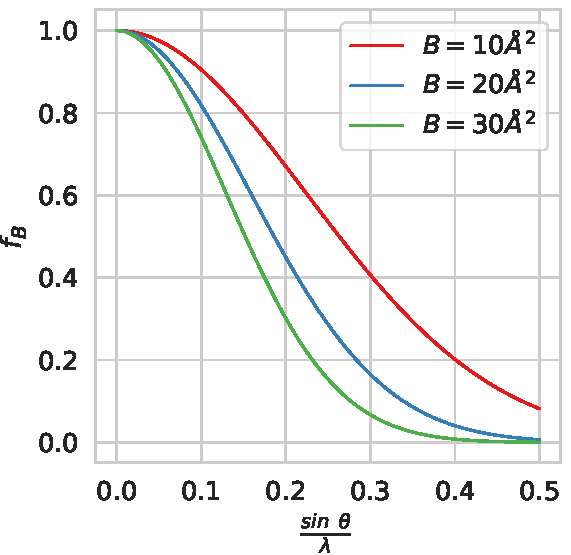
\includegraphics[width=0.5\textwidth]{chapters/Introduction/Figures/bfactors.pdf}
% \caption{\textbf{Attenuation of the incident waves due to increasing B-factor}. As B-factor increases, atomic scattering factor $(f)$ and consequently, the amplitude of wave scattered by an atom decreases rapidly.}%the List of Figures because of the *}
% \label{fig:bfactors}
% \end{figure}

Experimental B-factors for different residues in a protein sequence can be obtained the from Protein Data Bank (PDB). However, due to variation of structures, the B-factor of a given residue varies, even within the same polypeptide chain. For standardisation, the B-factor of residues within a chain are normalised using a z-score.

\begin{equation}
    B_{norm}^i =  \frac{B^i - \langle B\rangle}{\sigma}
\end{equation}

where, $B_{norm}^i$ is the normalised B-factor of residue $i$, $\langle B\rangle$ is the mean and $\sigma$ is the standard deviation of all B-factors across the chain.

\begin{wrapfigure}{r}{0.5\textwidth}
  \begin{center}
    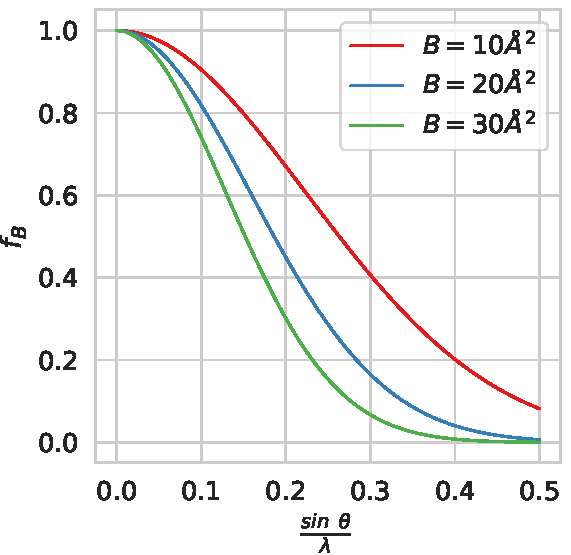
\includegraphics[width=0.45\textwidth]{chapters/Introduction/Figures/bfactors.pdf}
    \caption[Attenuation of the incident waves due to increasing B-factor.]{\textbf{Attenuation of the incident waves due to increasing B-factor.} As B-factor increases, atomic scattering factor $(f)$ and consequently, the amplitude of wave scattered by an atom decreases rapidly.}%the List of Figures because of the *}
    \label{fig:bfactors}
  \end{center}
\end{wrapfigure}


A number of high resolution structures are sampled from database and $B_{norm}^i$ is calculated for each residue on each protein. The mean of $B_{norm}^i$ across the sampled structures is the final normalised B-factor \cite{Schlessinger2005-ps, Smith2003-gb, Karplus1985-ea, vihinen1994accuracy}. 


The structural flexibility of protein can either be determined by using these normalised B-factors from experiments or by directly computing atomic displacements form molecular dynamics simulations (MDS) 
\cite{dong2018structural, kufareva2011methods}. Root mean square fluctuations and radius of gyration from MDS are useful in examining the flexibility. The profile plot (Fig. \ref{fig:hydrophobicity_flexibility_plot}) can be used to visualise and infer the local flexibility and dynamics of the protein structure. Since structural flexibility is inherently related to the protein dynamics, it is thought to influence several properties such as conformal variations, functions, thermal stability, ligand binding and disordered regions  \cite{Vihinen1987-jo, Teague2003-vq, Ma2005-cr, Yuan2005-gl, Yin2011-su, amaral2017protein}. Although the relationship of flexibility with solubility has been noted previously \cite{Tsumoto2003-qp}, it has been overlooked. 


% \begin{figure}[htbp!]
% \center
% 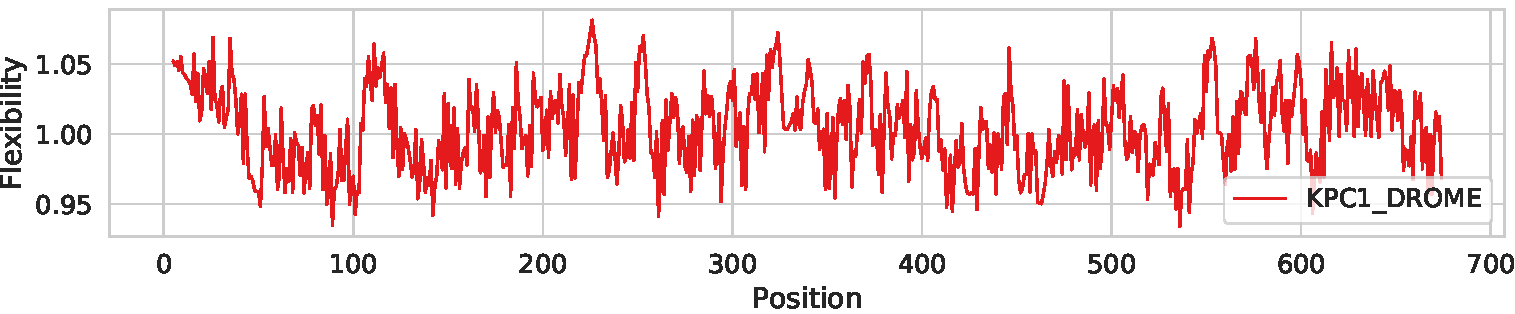
\includegraphics[width=1\textwidth]{chapters/Introduction/Figures/flexibility.pdf}
% \caption{\textbf{Flexibility profile of KPC1\_DROME (UniProtKB P05130)}. Plot was generated using normalised B-factors from Vihinen et al. (1994), with a sliding window of 9 residues. For these normalised B-factors, values greater than one are regarded to be flexible and values less than one are rigid. For illustration purposes, the residues at around position $440$ to $470$ are rigid, suggesting that there might be some structures. This is also supported by the hydropathy plot (Fig. \ref{fig:hydrophobicity_plot}) and the actual 3D structure (Fig. \ref{fig:3dplot_kpc1_drome}).}%the List of Figures because of the *}
% \label{fig:flexibility_plot}
% \end{figure}


Beside these features, amino acids also tend to have different structural propensities which is also thought to influence protein solubility \cite{Idicula-Thomas2005-qw, Huang2012-ft}.


Many solubility prediction tools have been developed around these features using statistical models (e.g., linear and logistic regressions) and machine learning models (e.g., support vector machines and neural networks) \cite{Hirose2013-nq, Habibi2014-jq, Hebditch2017-bg, Sormanni2017-lo, Heckmann2018-wb, Wu2019-nz, Yang2019-kd}. Newer tools such as SOLart also employ 3D structural information for a precise estimation of solvent accessibility, which makes the prediction more accurate \cite{hou2020solart}. Despite a higher prediction accuracy, the usability of these structure based tools might be limited due to the lack of 3D structure information of many proteins of interest.



